\documentclass[11pt]{article}

\usepackage{extras} % Se extras.sty

\begin{document}

\begin{titlepage}
\begin{center}

{\Large\bfseries TSEA56 - Kandidatprojekt i elektronik \\ LIPS Användarhandledning}
\begin{figure}[!htbp]
  \begin{center}
    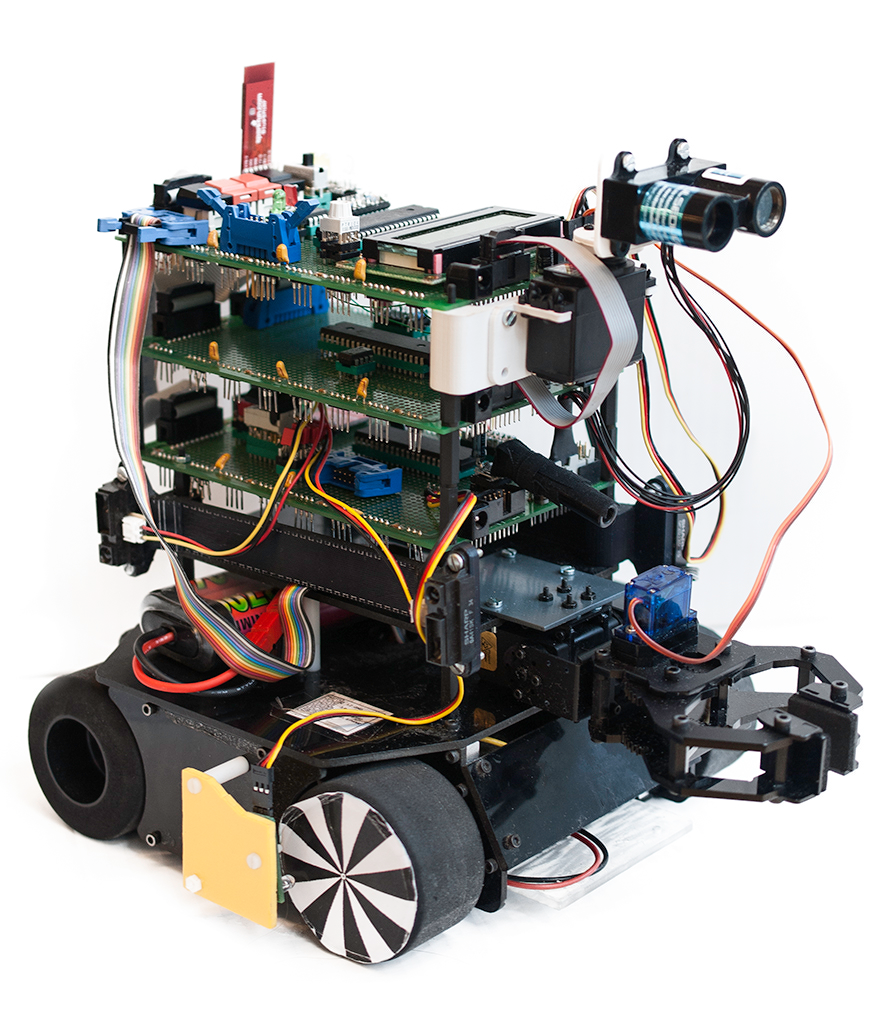
\includegraphics[scale=0.9]{images/RobotFront2.pdf}
  \end{center}
\end{figure}


  \begin{minipage}{0.5\textwidth}
    \centering
 Grupp 4 \\
\begin{tabular}{rl}
Hynén Ulfsjöö, Olle&\verb+ollul666+
\\
Wasteson, Emil&\verb+emiwa068+
\\
Tronje, Elena&\verb+eletr654+
\\
Gustafsson, Lovisa&\verb+lovgu777+
\\
Inge, Zimon&\verb+zimin415+
\\
Strömberg, Isak&\verb+isast763+
\\
\end{tabular}
\end{minipage}%
\begin{minipage}{0.5\textwidth}
  \centering
Version 1.0

\today
\vspace{2em}

Status
\begin{longtable}{|l|l|l|} \hline

Granskad & OHU & 2016-05-26 \\ \hline
Godkänd & - & - \\ \hline
 
\end{longtable}
\end{minipage}


\end{center}
\end{titlepage}


\pagebreak
\begin{center}

\section*{PROJEKTIDENTITET}
2016/VT, Undsättningsrobot Gr. 4

Linköpings tekniska högskola, ISY
\vspace{5em}

\begin{tabular}{|l|l|l|l|} \hline
\textbf{Namn} & \textbf{Ansvar} & \textbf{Telefon} & \textbf{E-post}  \\ \hline 
Isak Strömberg (IS) & Projektledare & 073-980 38 50 & isast763@student.liu.se \\ \hline
Olle Hynén Ulfsjöö (OHU)& Dokumentansvarig & 070-072 91 84 & ollul666@student.liu.se \\ \hline
Emil Wasteson (EW) & Hårdvaruansvarig & 076-836 61 66 & emiwa068@student.liu.se \\ \hline
Elena Tronje (ET) & Mjukvaruansvarig & 072-276 92 93 & eletr654@student.liu.se \\ \hline
Zimon Inge (ZI) & Testansvarig & 070-171 35 18 & zimin415@student.liu.se \\ \hline
Lovisa Gustafsson (LG) & Leveransansvarig & 070-210 32 53 & lovgu777@student.liu.se \\ \hline
\end{tabular}


E-postlista för hela gruppen: isast763@student.liu.se

\vspace{5em}
Kund: ISY, Linköpings universitet 
tel: 013-28 10 00, fax: 013-13 92 82 \\
Kontaktperson hos kund: Mattias Krysander \\
tel: 013-28 21 98, e-post: matkr@isy.liu.se \\

\vspace{5em}
Kursansvarig:  Tomas Svensson\\
tel: 013-28 13 68, e-post: tomass@isy.liu.se \\
Handledare: Peter Johansson \\
tel: 013-28 13 45, e-post: peter.a.johansson@liu.se
\end{center}
\pagebreak

\tableofcontents

\pagebreak

\section*{Dokumenthistorik}
\begin{table}[h]
\begin{tabular}{|l|l|l|l|l|} \hline

\textbf{Version} & \textbf{Datum} & \textbf{Utförda förändringar} & \textbf{Utförda av} & \textbf{Granskad} \\ \hline
1.0 & 2016-05-26 & Första utkastet & Grupp 4 & OHU \\ \hline
\end{tabular}
\end{table}

\pagebreak
\pagenumbering{arabic}

\section{Inledning}
Undsättningsroboten PigBot är en robot för undsättning av nödställda. Den autonoma konstruktionen gör att PigBot självständigt kan navigera och identifiera nödställda i en labyrint, utan att användarens ingripanden krävs.

Denna användarhandledning har för avsikt att ingående beskriva för användaren vilka användningsområden undsättningsroboten PigBot har. Här ges en ingående beskrivning hur PigBot kan kopplas samman med en extern datormodul samt hur det grafiska gränssnittet på datormodulen fungerar och bör användas. Användarhandledningen ska dessutom demonstrera hur hårdvaran på PigBot fungerar, detta ur ett användarmässigt perspektiv. 

För att bruka PigBot till fullo krävs en dator med möjligthet till parning via Bluetooth\textsuperscript{\circledR}. Om användaren förfogar över en dator som inte har denna möjlighet krävs dessutom en Bluetooth\textsuperscript{\circledR}-adapter för att kunna ansluta till PigBot.

\subsection{Förkortningar}
Denna användarhandledning kommer tillämpa förkortningar för att ge användaren bättre översikt i sin handledning. Samtliga förkortningar är listade nedan:

\begin{itemize}
  \item[-] GUI - Står för \textit{Graphical User Interface} vilket är engelska för grafiskt användargränssnitt. Detta är den mjukvara som ska underlätta interaktionen mellan användaren och PigBot.
\end{itemize}

\pagebreak

\section{Roboten}
Nedan följer en användarhandledning för själva roboten. Kapitlet är uppdelat i två delar. Dioder och brytare beskriver de fysiska komponenter som är monterade på roboten. Styrning ger en förklaring till hur roboten ska användas i autonomt respektive manuellt läge.

\subsection{Dioder, brytare och display}
Hädanefter numreras dioder och brytare enligt figur \ref{picTop} och nedan följer en förklaring av respektive.

\begin{figure}[htbp]
	\centering
	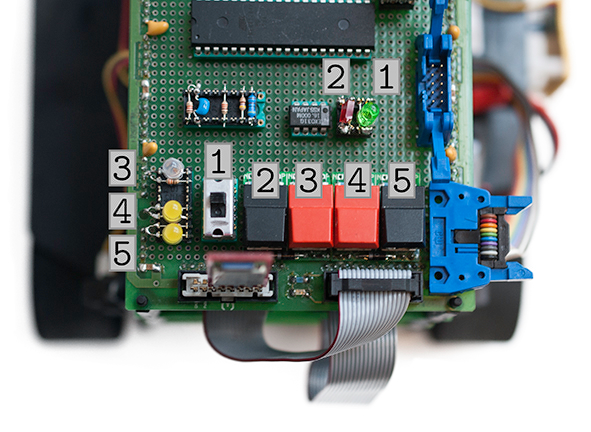
\includegraphics[scale=1]{Images/RobotTopInfo.pdf}
	\caption{\textit{Illustration av PigBots olika tryckknappar och dioder.} \label{picTop}}
\end{figure}

De dioder som är placerade på robotens övre modul visar båda styrläge och status under uppdraget.
\begin{description}[style=unboxed, leftmargin=0cm]
  \item[Diod 1] visar ifall roboten befinner sig i autonomt eller manuellt läge. 
    \begin{itemize}
      \setlength\itemsep{-0.5em}
      \item[-] På: Autonomt läge 
      \item[-] Av: Manuellt läge
    \end{itemize}
  \item[Diod 2] visar ifall roboten befinner sig i \textit{debug}-läge läge eller inte.
    \begin{itemize}
      \setlength\itemsep{-0.5em}
      \item[-] På: \textit{debug}-läge
      \item[-] Av: Vanligt läge
    \end{itemize}
  \item[Diod 3] visar ifall roboten är klar med uppdraget eller inte.
    \begin{itemize}
      \setlength\itemsep{-0.5em}
      \item[-] På: Roboten är klar med uppdraget
      \item[-] Av: Roboten är ännu inte klar med uppdraget
    \end{itemize}
  \item[Diod 4 och 5] visar tillsammans statusen för roboten under uppdragets genomförande. Dioderna räknas upp binärt i takt med att ett moment har avklarats. Diod 5 är mest signifikant bit. De möjliga kombinationer som dioderna kan anta och dess beskrivning återfinns nedan.

    \hspace{2em}\begin{tabular}{c c p{8cm}}
	Diod 5 & Diod 4 & Beskrivning \\ \hline
	Av & Av & Väntar på startkommando \\
	Av & På & Söker efter målet \\
	På & Av & Har funnit målet och återkommit till startposition. Gripklon inväntar en förnödenhet. \\
	På & På & Klon är stängd och roboten är redo för att färdas kortaste vägen till målet.

    \end{tabular}
\end{description}

De brytare som finns kopplade på robotens övre modul nollställer robotens moduler eller skickar ett startkommando. 
\begin{description}[style=unboxed, leftmargin=0cm]
  \item[Brytare 1] Sätter roboten i autonomt eller manuellt läge. 
    \begin{itemize}
      \setlength\itemsep{-0.5em}
      \item[-] Föröver: Autonomt läge
      \item[-] Akteröver: Manuellt läge
    \end{itemize}
  \item[Brytare 2] används inte.
  \item[Brytare 3] nollställer styrmodulen, det översta virkortet.
  \item[Brytare 4] nollställer huvudmodulen, det mellersta kortet.
  \item[Brytare 5] skickar ett startkommando till roboten.
\end{description}

Roboten initieras genom att aktivera brytarna i ordningen ($3 \rightarrow 4 \rightarrow 5$).

Utöver dioder och brytare finns även en LCD-display monterad på det övre kortet. LCD-displayen visar information om måldetektion, främre sensorvärde och tillryggalagd sträcka enligt figur \ref{lcd}.

\begin{figure}[htbp]
	\centering
	\documentclass[border=10px]{standalone}
\usepackage{tikz}
\usetikzlibrary{patterns}
\usetikzlibrary{shapes.arrows}
\usepackage{amssymb}
\usetikzlibrary{calc}
\usepackage{verbatim}
\usetikzlibrary{positioning}
\tikzset{sign/.style={black, inner sep = 0pt, minimum width = 0mm, text width = 5mm, fill=green!20, font=\bfseries,  minimum height = 8mm,  align = center}}
\usepackage{lcd}
\begin{document}
	
\begin{tikzpicture}[scale=1]
  \draw[draw = black] (-0.8,1) rectangle (10,-2); 
  \node[sign] (n0) {};
  \foreach \x/\t [remember=\x as \lastx (initially 0)] in {1/ , 2/ , 3/ , 4/T , 5/A , 6/R , 7/G , 8/E , 9/T , 10/: , 11/0 , 12/ , 13/ , 14/ , 15/}{
    \node[sign, right = 1mm of n\lastx] (n\x) {\t};
  }

  \node[sign, below = 1mm of n0] (m0) {F};
  \foreach \x/\t [remember=\x as \lastx (initially 0)] in {1/O, 2/R, 3/W, 4/:, 5/1, 6/2 , 7/3, 8/ , 9/T, 10/R, 11/I, 12/P, 13/:, 14/4, 15/5}{
  \node[sign, right = 1mm of m\lastx] (m\x) {\t};
}


\end{tikzpicture}
	
\end{document}

	\caption{\textit{LCD-displayen under färd} \label{lcd}}
\end{figure}

\begin{description}[style=unboxed, leftmargin=0cm]
  \item[Target] visar ifall roboten, för tillfället, set målet framför sig.
  \item[Forw] visar det avstånd roboten har rakt föröver till nästa vägg i centimeter.
  \item[Trip] visar den totala tillryggalagda sträckan i meter.
\end{description}

För att justera kontrasten på LCD-displayen används den potentiometer som syns i bild \ref{lcdPot}. Om LCD-displayen inte visar någon information trots att roboten är aktiv, justera då kontrasten.


\begin{figure}[htbp]
	\centering
	\includegraphics[scale=1]{images/RobotLCD.pdf}
	\caption{\textit{LCD-displayen med tillhörande potentiometer} \label{lcdPot}}
\end{figure}



\subsection{Styrning}
Roboten används autonomt genom att följa instruktionerna nedan.
\begin{enumerate}
    \renewcommand*\labelenumi{\theenumi\vspace{1pt} - }
  \item Koppla på ett laddat batteri med spänningsnivå $7.2$ V och slå på batterispänningen.
  \item Slå över brytare 1 till autonomt läge.
    \renewcommand*\labelenumi{\hspace{1pt} (\theenumi)\vspace{1pt} - }

  \item Valfritt: Koppla upp mot roboten med en dator.
    \renewcommand*\labelenumi{\theenumi\vspace{1pt} - }
  \item Nollställ roboten genom att aktivera brytarna 3 och 4 i den ordningen. Nu ska endast diod 1 vara aktiv.
  \item Placera roboten vid labyrintens start och aktivera brytare 5. 
  \item När roboten har identifierat målet, återkommit till startposition och öppnat gripklon ska ett objekt placeras däremellan och brytare 5 aktiveras.
  \item Aktivera brytare 5 för att roboten ska navigera till målet och släppa objektet. 
\end{enumerate}

För manuell körning krävs det att brytare 1 är inställd rätt och att roboten är uppkopplad mot en datormodul. Följ därefter de kortkommandon som finns i avsnitt \ref{shortcuts}.


\section{Datormodul}
Detta kapitel behandlar det GUI som medföljer PigBot. Gränssnittet är fristående från robototen och körs på användarens externa datormodul.

\subsection{Grafiskt gränssnitt}
Datormodulens GUI är indelat i fem olika delar: en meny, en kartpanel, en tabellpanel, en grafpanel och robotens statuspanel. Figur \ref{DebugOff} visar programmet i sin helhet.

\begin{figure}[htbp]
	\centering
	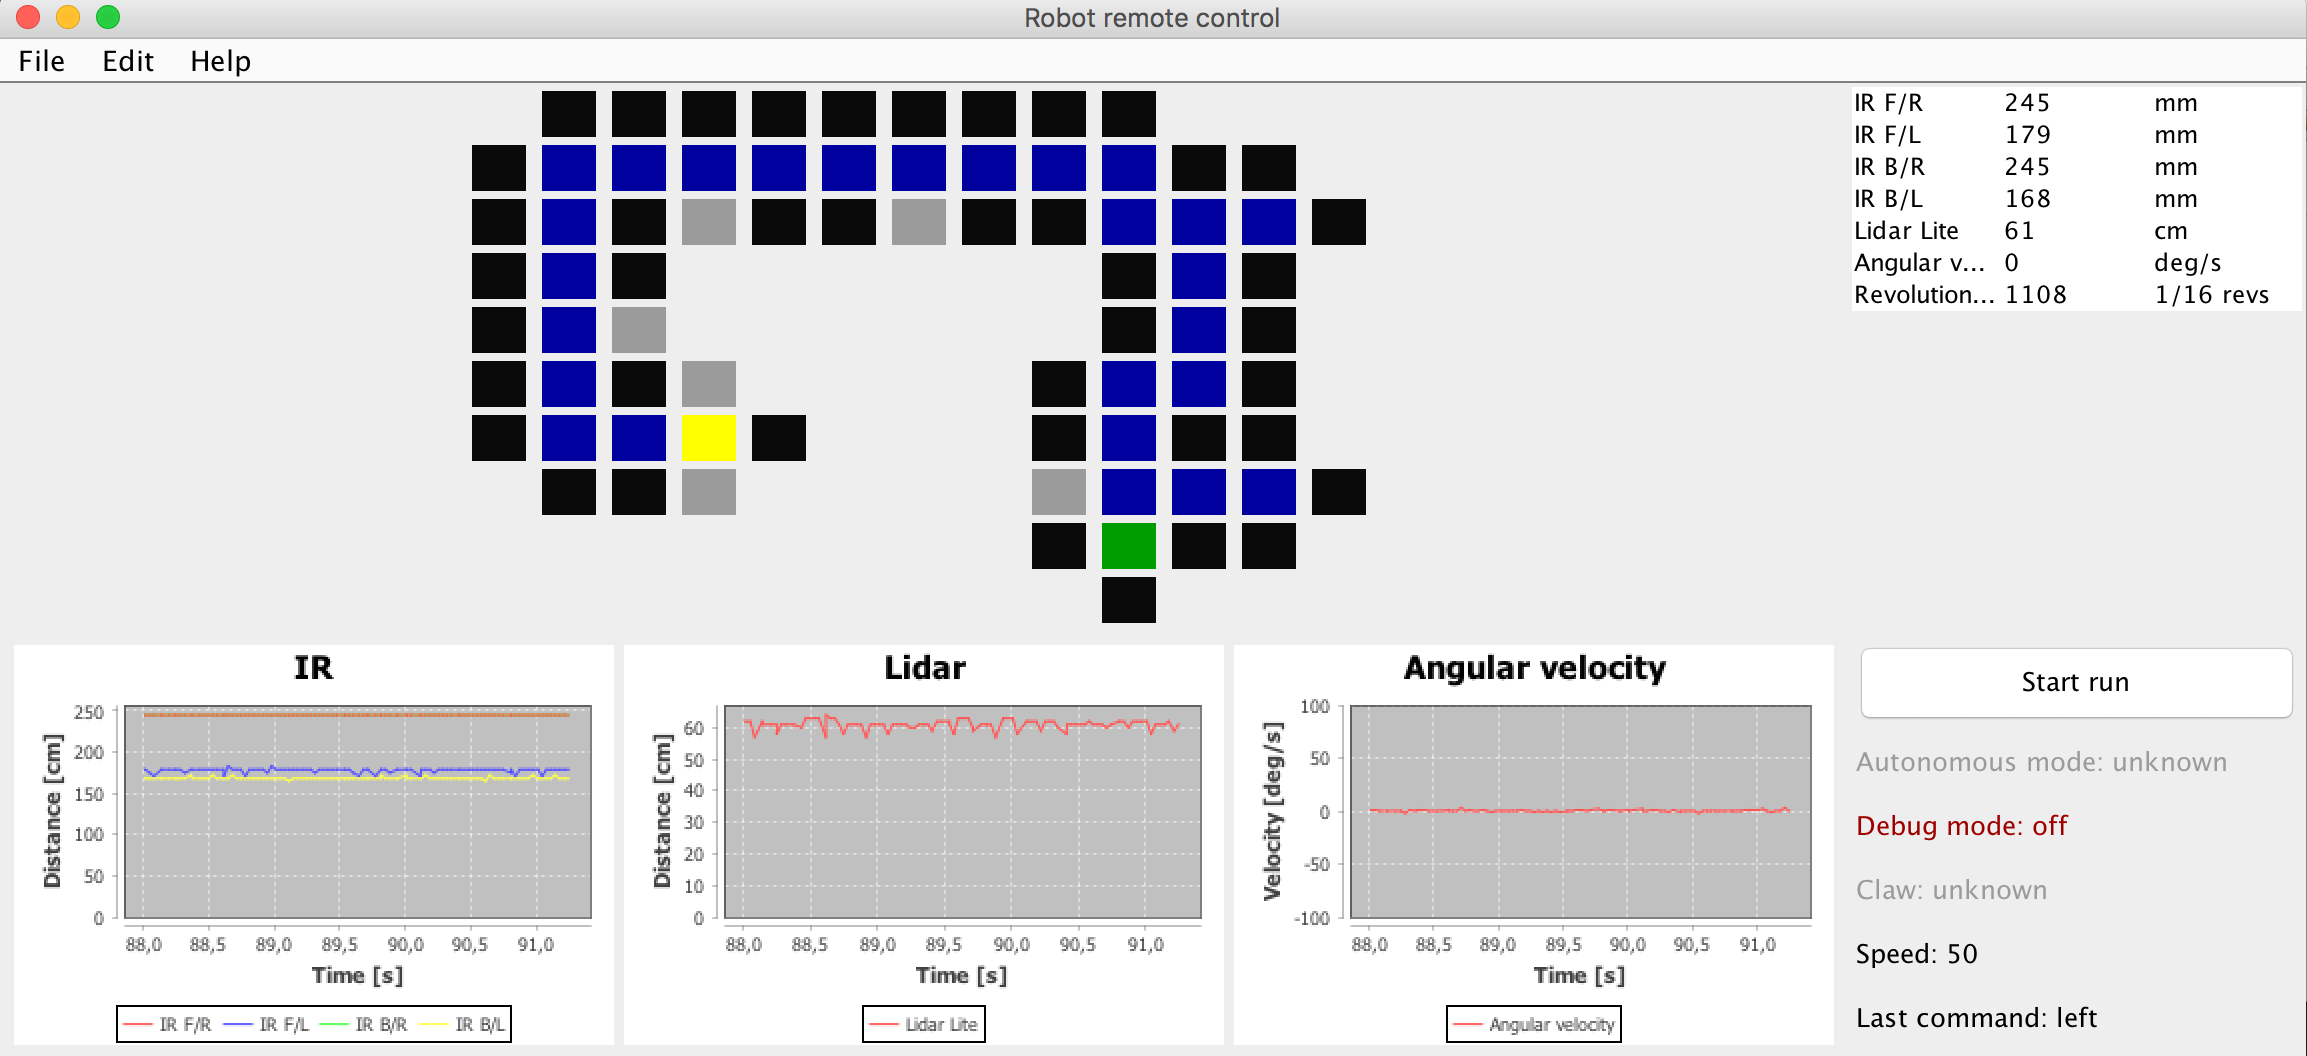
\includegraphics[scale=0.35]{Images/computerDebugOff}
	\caption{\textit{GUI med tillhörande paneler efter rutt i ett bansystem.} \label{DebugOff}}
\end{figure}

\subsubsection{Meny} Låter användaren justera olika inställningar för programmet. Under fliken \emph{File}  finns:
\begin{description}
  \item[Save log] - sparar nuvarande loggfil och öppnar en ny (endast tillgänglig i \textit{debug}-läge).
  \item[Comment log] - sparar en kommentar till nuvarande loggfil (endast tillgänglig i \textit{debug}-läge).
	\item[Select serial port] - låter användaren välja vilken serieport programmet ska använda.
	\item[Connect to selected port] - kopplar upp mot den valda serieporten. Kopplar upp mot en förprogrammerad port om inte en annan port valts. 
\end{description}

Under fliken \emph{Edit} finns:
\begin{description}
  \item[Debug mode] - väljer \textit{debug}-läge av/på (endast tillgänglig i autonomt läge).
	\item [Clear map] - rensar programkartan (påverkar inte robotens interna karta).
\end{description}

Utöver oven nämnda två finns även en hjälpmeny där användaren kan komma åt användarhandledningen och öppna en lista över alla tangentbordsgenvägar.

\paragraph{Kartpanel} Visar alla de moduler som roboten har besökt samt alla intilligande moduler. Innan startad körning är alltså kartan blank. Modulerna representeras med olika färger beroende på deras egenskaper:
\begin{itemize}
  \item[-] \makebox[1cm][l]{Grön} - modulen där körningen startade.
  \item[-] \makebox[1cm][l]{Röd} - modulen där målet identifierats.
  \item[-] \makebox[1cm][l]{Blå} - utforskad, öppen modul.
  \item[-] \makebox[1cm][l]{Gul} - robotens nuvarande position.
  \item[-] \makebox[1cm][l]{Svart} - väggmodul.
  \item[-] \makebox[1cm][l]{Grå} - outforskad, öppen modul.
\end{itemize}

\paragraph{Tabellpanel} Visar de senaste mottagna sensorvärdena för alla sensorer. I \textit{debug}-läge visas även en tabell där användaren kan ändra vissa parametrar hos roboten. Dessa ändras genom att ändra tabellvärdet och trycka Enter.

\paragraph{Grafpanel}
Visar tre grafer med  de senaste 100 mottagna mätvärdena från:
\begin{itemize}
  \item[-] Sidledes avståndssensorer,
  \item[-] Främre avståndssensor,
  \item[-] Rotationshastighet.
\end{itemize}

\paragraph{Robotens statuspanel}
Innehåller information om robotens olika tillstånd och lägen. Är roboten i autonomt läge visas även en knapp \emph{Start run} som låter användaren starta en körning. Är roboten i \textit{debug}-läge visas även en \emph{Next decision} som aktiverar nästa styrbeslut hos roboten. 

\subsection{Övrigt}
\label{shortcuts}
\paragraph{Systemkrav} För att köra programmet krävs Java 1.8 samt en hårdvaruenhet för Bluetooth\textsuperscript{\circledR}-kommunikation.
\paragraph{Kortkommandon}\label{kortkommandon}
\begin{description}
	\item[W] - kör roboten framåt (fungerar endast i manuellt läge).
	\item[A] - roterar roboten åt vänster (fungerar endast i manuellt läge).
	\item[S] - kör roboten bakåt (fungerar endast i manuellt läge).
	\item[D] - roterar roboten åt vänster (fungerar endast i manuellt läge).
	\item[C] - öppnar/stänger robotens klo (fungerar endast i manuellt läge).
\end{description}


\end{document}
